\documentclass[wide]{beamer}
\usetheme{Pittsburgh}
\usepackage{listings}
\usepackage[utf8x]{inputenc}
\usepackage{etex}
\usepackage[setrelation]{math}
\usepackage[modernsign,substopindex,shortmquant,mquantifiertype,
mconnectiveformal,postfixflatinterpret,bracketmodalinterpret,
setfixinterpret,modifopindex,seqinfers,seqoptional,footnotecalculus,abbrseqcontext,shortterms,nosigmaterms,novarterms]{logic}
\usepackage[pretest,nocommandblocks]{progreg}
\usepackage[bracketinterpret,postfixinterpret,bracketmodalinterpret,simplenames]{dL}
\usepackage{tabularx,xcolor,colortbl}
\usepackage{booktabs}
\usepackage{todonotes}
\usepackage{wrapfig}
\usepackage{stmaryrd}
\usepackage{proof}
\usepackage{prettyref}
\usepackage{tikz}
\usepackage{pgfplots}
\usepackage{slidetool}
\usepackage{marvosym}
\usenavigationsymbolstemplate{}
\pgfplotsset{width=8cm,compat=1.9}
 \usetikzlibrary{arrows}
 \usetikzlibrary{calc}
 \usetikzlibrary{fit}
 \usetikzlibrary{positioning,shadows}
 \usetikzlibrary{automata}
 \usetikzlibrary{shapes,arrows}
 \usetikzlibrary{decorations.text}
 \usetikzlibrary{decorations.markings}
 \usetikzlibrary{trees,snakes}
\usetikzlibrary{pgfplots.dateplot}
\usepackage{relsize}
\tikzset{fontscale/.style = {font=\relsize{#1}}}
\usepackage{pgfplotstable}
\usepackage{filecontents}

\definecolor{vermillion}{rgb}{0.8,0.4,0}
\definecolor{myblue}{rgb}{0,0.45,0.7}
\definecolor{myyellow}{rgb}{0.85,0.8,0.17}


\newcommand{\rref}[2][]{\prettyref{#2}}

  \tikzstyle{noteline}=[shorten <=8pt]%
  \tikzstyle{notebox}+=[minimum height=1.1cm]%
\newrefformat{sec}{Section\,\ref{#1}}
\newrefformat{appendix}{Appendix\,\ref{#1}}
 \newrefformat{model}{Model\,\ref{#1}}
 \newrefformat{listing}{Listing\,\ref{#1}}
 \newrefformat{line}{line\,\ref{#1}}
 \newrefformat{def}{Definition\,\ref{#1}}
 \newrefformat{defn}{Definition\,\ref{#1}}
 \newrefformat{thm}{Theorem\,\ref{#1}}
 \newrefformat{ax}{\ref{#1}}
 \newrefformat{prop}{Proposition\,\ref{#1}}
 \newrefformat{lem}{Lemma\,\ref{#1}}
 \newrefformat{cor}{Corollary\,\ref{#1}}
 \newrefformat{ex}{Example\,\ref{#1}}
 \newrefformat{tab}{Table\,\ref{#1}}
 \newrefformat{fig}{Figure\,\ref{#1}}
 \newrefformat{eqn}{(\ref{#1})}
\renewcommand{\ivr}{\psi}
\providecommand{\tweak}[1]{#1}
\newcommand{\untweak}[1]{}
\newcommand{\ignore}[1]{}
\newcommand{\stdI}{\dLint[state=\nu]}%
\newcommand{\ws}{\nu}
\newcommand{\wt}{\omega}%
\newcommand{\I}{\iconcat[state=\ws]{\stdI}}%
\newcommand{\It}{\iconcat[state=\wt]{\stdI}}%
\definecolor{vgray}{rgb}{.35,.35,.35}
\renewcommand*{\irrulename}[1]{\text{\textcolor{vgray}{\upshape#1}}}
\usepackage{tikz}
\usepackage{stmaryrd}
\usetikzlibrary{arrows,matrix}
\newcommand{\isabelle}{Isabelle/HOL\xspace}
\newcommand{\allstate}{\mathcal{S}}
\newcommand{\tvm}{\oslash}
\newcommand{\tvt}{\oplus}
\newcommand{\tvf}{\ominus}
\newcommand{\term}{\mathbf{Term}\xspace}
\newcommand{\lequiv}{\leftrightarrow}
\newcommand{\state}{\mathbf{State}\xspace}
\newcommand{\prop}{\mathbf{Prop}\xspace}
\newcommand{\fml}{\mathbf{Fml}\xspace}
\newcommand{\dLi}{\ensuremath{\dL_{\iota}}\xspace}
\newcommand{\KeY}{KeY}
\newcommand{\tint}[2]{#2\lenvelope#1\renvelope}
\newcommand{\fint}[2]{#2\lenvelope#1\renvelope}
\newcommand{\pint}[1]{\lenvelope#1\renvelope}
\newcommand{\piint}[2]{#2\lenvelope#1\renvelope}
\newcommand{\meps}[2]{\iota{#1}\,{#2}}
\newcommand{\mepsIndef}[2]{\varepsilon{#1}\,{#2}}
\newcommand{\R}{\mathbb{R}}
\newcommand{\err}{\textsf{Err}\xspace}
\newcommand{\ffalse}{\textsf{false}\xspace}
\newcommand{\ftrue}{\textsf{true}\xspace}
\newcommand{\projGen}[2]{\ensuremath{\pi_{#1}}{#2}}
\newcommand{\projL}[1]{\projGen{1}{#1}}
\newcommand{\projR}[1]{\projGen{2}{#1}}
\newcommand{\inR}[1]{\textsf{in}{\ensuremath{\mathbb{R}}}(#1)}
\newcommand{\isT}[1]{\textsf{isT}(#1)}
\newcommand{\om}{\omega}
\newcommand{\tom}{\tilde{\omega}}
\newcommand{\tnu}{\tilde{\nu}}
\newcommand{\tmu}{\tilde{\mu}}
\newcommand{\denote}[1]{\mathsf{E}(#1)}
\newcommand{\llc}[3]{\mathsf{LLC}(#2(#1))}
\newcommand{\cont}[2]{\mathsf{Con}(#2(#1))}
\newcommand{\tder}[2]{\der{#2(#1)}}
\newcommand{\hasdiff}[1]{\mathsf{D}(#1)}
\newcommand{\vepsilon}{\xi}
\newcommand{\stepsto}{\allowbreak\mapsto\allowbreak}
\newcommand{\bebecomes}{\mathrel{::=}}
\newcommand{\alternative}{~|~}
\newcommand{\ModelPlex}{ModelPlex\xspace}
\providecommand{\KeYmaeraX}{KeYmaera X\xspace}


% CdGL
\newcommand{\GL}{GL\xspace}
\newcommand{\CdGL}{CdGL\xspace}
\newcommand{\dRL}{dRL\xspace}


\newcommand{\engineer}[1][1in]{\includegraphics[width=#1]{img/rosie.png}}
\newcommand{\logician}[1][1in]{\includegraphics[width=#1]{img/hilbert.png}}
\newcommand{\logicuser}[1][1in]{\includegraphics[width=#1]{img/hamilton.png}}


\newcommand{\speak}[2]{\small\begin{minipage}{1.3in}{#1}{#2}\end{minipage}}
\newcommand{\say}[1]{\speak{#1}{}}
\newcommand{\sayHappy}[1]{\speak{#1}{\Smiley}}
\newcommand{\saySad}[1]{\speak{#1}{\Frowny}}
\newcommand{\turn}{\textsc{Turn}}
\newcommand{\nim}{\textsc{Nim}}
\newcommand{\cake}{\textsc{CC}}


\newcommand{\rangevar}{\textsf{Range}}
\newcommand{\testvar}{\textsf{test}}
\newcommand{\elem}[2]{\textsf{Dec}[#1](#2)}
\newcommand{\spc}{\hspace{0.15in}}
\newcommand{\kwmod}{\textsf{mod}}
\newcommand{\emod}[2]{#1~\kwmod~#2}
\newcommand{\kwdiv}{\textsf{div}}
\newcommand{\ediv}[2]{#1~\kwdiv~#2}
\newcommand{\kwsig}{\Sigma}
\newcommand{\sig}[1]{\kwsig(#1)}
\newcommand{\interp}{I}
\newcommand{\valset}[1]{\mathfrak{V}(#1)}
\newcommand{\kwbool}{\m{\mathbb{B}}}
\newcommand{\kwint}{\m{\mathbb{Z}}}
\newcommand{\kwreal}{\m{\mathbb{R}}}
\newcommand{\kwintsig}{\Xi}
\newcommand{\intsig}[1]{\kwintsig(#1)}
\newcommand{\churchkleene}{\omega_{\text{CK}}}
\newcommand{\restL}[1]{#1_L}
\newcommand{\restR}[1]{#1_R}
\newcommand{\apL}[1]{#1_{\langle{0}\rangle}}
\newcommand{\apR}[1]{#1_{\langle{1}\rangle}}
\newcommand{\dpL}[1]{#1_{[0]}}
\newcommand{\dpR}[1]{#1_{[1]}}

\newcommand{\va}{a}
\newcommand{\vb}{b}
\newcommand{\vca}{\overline{a}}
\newcommand{\vcb}{\overline{b}}

\newcommand{\btt}{\texttt{tt}}
\newcommand{\bff}{\texttt{ff}}
\newcommand{\stt}{\top}
\newcommand{\sff}{\bot}
\newcommand{\demonactive}[2]{\textrm{aD}(#1,#2)}
\newcommand{\demondormant}[2]{\textrm{dD}(#1,#2)}
\newcommand{\sren}[3]{\urename[{#1}]{#2}{#3}}%{\subst[{#1}]{#2}{#3}}
\newcommand{\ssub}[3]{\subst[{#1}]{#2}{#3}}
\newcommand{\eren}[3]{\urename[{#1}]{#2}{#3}}%{\subst[{#1}]{#2}{#3}}
\newcommand{\earen}[2]{\urename[{#1}]{\boundvars{#2}}{\vec{y}}}%{\subst[{#1}]{\boundvars{#2}}{\vec{y}}}

\newcommand{\allcon}{\allregion}
\newcommand{\somesemi}[2]{\epsilon #1~|~#2}

\newcommand{\rzF}[2]{#1 \vdash #2}
\newcommand{\rzA}[3]{\langle{#2}\rangle(#1)=(#3)}
\newcommand{\rzD}[3]{[{#2}](#1)=(#3)}
\newcommand{\rzFst}[1]{#1_0}
\newcommand{\rzSnd}[1]{#1_1}
\newcommand{\rzThd}[1]{#1_2}
\newcommand{\rzFrt}[1]{#1_3}
\newcommand{\rzApp}[2]{#1\,#2}
\newcommand{\sa}{\omega}
\renewcommand{\sb}{\nu}
\newcommand{\Sc}{\mu}
\renewcommand{\aa}{a}
\newcommand{\ab}{b}
\newcommand{\ac}{c}
\newcommand{\da}{d}
\newcommand{\db}{D}
\newcommand{\dc}{\DJ}
\newcommand{\allRz}{\mathcal{R}\mathbf{z}}
\newcommand{\rzfor}[1]{#1\,\allRz}

\newcommand{\mto}{\rightharpoonup}
\newcommand{\esub}[3]{[{#3}/{#2}]{#1}}
\newcommand{\tsub}[3]{\subst[#1]{#2}{#3}}


%\newcommand{\rzF}[2]{#1 \vdash #2}
%\newcommand{\rzA}[3]{\langle{#2}\rangle(#1)=(#3)}
%\newcommand{\rzD}[3]{[{#2}](#1)=(#3)}
\newcommand{\rzNil}{\epsilon}
\newcommand{\rzCons}[2]{(#1,#2)}
\newcommand{\rzBLam}[2]{\lambda #1:\allstate.~#2}
\newcommand{\rzHOLam}[3]{\Lambda #1:\rzfor{#2}.~#3}
\newcommand{\rzFOLam}[3]{\Lambda #1:#2.~#3}
%\newcommand{\rzApp}[2]{#1\,#2}
\newcommand{\fintR}[1]{\fint{#1}{}} %{#1#2}
\newcommand*{\strategyforR}[2][]{{#2}\Langle{#1}\Rangle}
\newcommand*{\istrat}[3][]{\strategyforR[#1]{#2}^{#3}}

\newcommand*{\dstrategyforR}[2][]{{#2}\lenvelopewide{#1}\renvelopewide}
%{{#2}\llbracket{#1}\rrbracket}
\newcommand*{\idstrat}[3][]{\dstrategyforR[#1]{#2}^{#3}}
\newcommand{\cint}[1]{\fint{\bigwedge #1}}
\newcommand{\cintR}[1]{\fintR{\bigwedge #1}}
\newcommand{\seq}[2]{#1 \vdash #2}
\newcommand{\proves}[3]{#1\allowbreak\vdash #2 \allowbreak \mathop{:} #3}

\newcommand{\edOpencons}{\langle}
\newcommand{\edClosecons}{\rangle}
\newcommand{\edSepcons}{,}
\newcommand{\edcons}[2]{\edOpencons{#1}\edSepcons{#2}\edClosecons}
%\newcommand{\edcons}[2]{\langle#1,#2\rangle}
\newcommand{\ebOpencons}{[}
\newcommand{\ebSepcons}{,}
\newcommand{\ebClosecons}{]}
\newcommand{\ebcons}[2]{\ebOpencons#1\ebSepcons#2\ebClosecons}
\newcommand{\eCons}[2]{\lstrike{#1,#2}\rstrike}
\newcommand{\eSnoc}[2]{\llensehat{#1,#2}\rlensehat}
\newcommand{\pmodality}[2]{\llensehat{#1}\rlensehat{#2}}
\newcommand{\econs}[2]{\eCons{#1}{#2}}
\newcommand{\einjL}[1]{\ell \cdot #1}
\newcommand{\einjR}[1]{r \cdot #1}
\newcommand{\kwcase}{\textrm{case}}
\newcommand{\ecaseHead}[1]{\langle\kwcase\textrm{ }#1{\text{\textrm{ of }}}}
\newcommand{\ecaseLeft}[2]{#1\Rightarrow~#2}
\newcommand{\ecaseRight}[2]{~|~#1\Rightarrow~#2}
\newcommand{\ecaseEnd}{\rangle}
\newcommand{\ecasegen}[5]{\ecaseHead{#1}\allowbreak\ecaseLeft{#2}{#3}\allowbreak\ecaseRight{#4}{#5}\ecaseEnd}
\newcommand{\ecase}[3]{\ecasegen{#1}{\ell}{#2}{r}{#3}}
\newcommand{\edcase}[3]{\ecase{#1}{#2}{#3}}
\newcommand{\ercase}[3]{\langle\textrm{case}_*\ #1\text{ of }\pvs\Rightarrow~#2~|~\pvg\Rightarrow#3\rangle}
\newcommand{\eCase}[3]{\lstrike\kwcase\textrm{ }#1\textrm{ of }\allowbreak\ell\Rightarrow~#2~\allowbreak|~r\Rightarrow~#3\rstrike} %\{\textrm{case}\}\ #1\textrm{ of }\ell.~#2~|~r.~#3

\newcommand{\edinjL}[1]{\langle\ell \cdot #1\rangle}
\newcommand{\edinjR}[1]{\langle r \cdot #1\rangle}
\newcommand{\eInjL}[1]{\lstrike\ell \cdot #1\rstrike}
\newcommand{\eInjR}[1]{\lstrike{r \cdot #1}\rstrike}
\newcommand{\kwrep}{\textrm{rep}}
\newcommand{\erep}[3]{{#1}\textrm{ }\kwrep\text{ }#3.~{#2}}
\newcommand{\eapp}[2]{#1\ #2}
\newcommand{\elamgen}[3]{\lambda #1:#2.~ #3}
\newcommand{\eplam}[2]{\elamgen{\pvx}{#1}{#2}}
\newcommand{\etlam}[2]{\elamgen{x}{#1}{#2}}
\newcommand{\ebseq}[1]{[\iota~#1]}
\newcommand{\ebseqinv}[1]{[\iota~{#1}^{-1}]}
\newcommand{\edseq}[1]{\langle\iota~#1\rangle}
\newcommand{\edseqinv}[1]{\langle\iota~{#1}^{-1}\rangle}
\newcommand{\eSeq}[1]{\lstrike\iota~#1\rstrike}
\newcommand{\eSeqinv}[1]{\lstrike\iota~{#1}^{-1}\rstrike}
\newcommand{\ebOpenswap}{[\textrm{yield }}
\newcommand{\ebCloseswap}{]}
\newcommand{\ebswap}[1]{\ebOpenswap#1\ebCloseswap}
\newcommand{\edOpenswap}{\langle\textrm{yield }}
\newcommand{\edCloseswap}{\rangle}
\newcommand{\edswap}[1]{\edOpenswap#1\edCloseswap}
%\llensehat \rlensehat  \lstrike \rstrike
\newcommand{\eSwap}[1]{\lstrike\textrm{yield }#1\rstrike}
\newcommand{\ePaws}[1]{\llensehat\textrm{yield }#1\rlensehat}
\newcommand{\emonInfix}[1]{{\circ_{#1}}}
\newcommand{\emon}[3]{{#1} \emonInfix{#3} {#2}}
%\newcommand{\eQEpos}{\textrm{QE}_{pos}}
%\newcommand{\eQEneg}{\textrm{QE}_{neg}}
\newcommand{\eQE}[2]{\textsf{FO}[#1](#2)}
%\newcommand{\eQEN}[1]{\textsf{QE}[#1]_\mathbb{N}}
%\newcommand{\eQER}[1]{\textsf{QE}[#1]_\mathbb{R}}
\newcommand{\emetsplit}{\textrm{split}\met}
\newcommand{\esplit}[3]{\textrm{split }{[#1\sim#2]}~#3}
\newcommand{\kwstop}{\textrm{stop}}
\newcommand{\kwgo}{\textrm{go}}
\newcommand{\estop}[1]{\langle\kwstop\ #1\rangle}
\newcommand{\ego}[1]{\langle\kwgo\ #1\rangle}
\newcommand{\kwroll}{\textrm{roll}}
\newcommand{\kwunroll}{\textrm{unroll}}
\newcommand{\ebroll}[1]{[\kwroll\ {#1}]}
\newcommand{\ebunroll}[1]{[\kwunroll\ #1]}
\newcommand{\eRoll}[1]{\lstrike\kwroll\ #1\rstrike}
\newcommand{\eUnroll}[1]{\lstrike\kwunroll\ #1\rstrike}
\newcommand{\eghost}[4]{\textrm{Ghost}[#1=#2](#3.~#4)}
\newcommand{\eAsgn}[4]{\lstrike\humod{#2}{\eren{f}{#2}{#1}}\text{ in }#3.~#4\rstrike}
\newcommand{\eAsgneq}[4]{\eAsgn{#1}{#2}{#3}{#4}}
\newcommand{\etconsgen}[5]{\langle{\eren{#4}{#1}{#2}}~{{:}{*}}~#3.~#5\rangle}
\newcommand{\etcons}[2]{\etconsgen{x}{y}{\pvx}{#1}{#2}}
\newcommand{\ietcons}[3]{\langle{\eren{#2}{#1}{~}}~{{:}{*}}~#3\rangle}

\newcommand{\ebasgneq}[4]{[\humod{#2}{\eren{f}{#2}{#1}}\text{ in }#3.~#4]}
\newcommand{\edasgneq}[4]{\langle\humod{#2}{\eren{f}{#2}{#1}}\text{ in }#3.~#4\rangle}
\newcommand{\edasgn}[4]{\edasgneq{#1}{#2}{#3}{#4}}
\newcommand{\ebasgn}[4]{\ebasgneq{#1}{#2}{#3}{#4}}
\newcommand{\iebasgn}[2]{[\humod{#1}{\eren{f}{#1}{~}}\text{ in }~#2]}
\newcommand{\iedasgn}[2]{\langle\humod{#1}{\eren{f}{#1}{~}}\text{ in }~#2\rangle}
%\newcommand{\iedasgn}[2]{\edasgneq{~}{#1}{#1}{#2}}
%\newcommand{\iebasgn}[2]{\ebasgneq{~}{#1}{#1}{#2}}

\newcommand{\eunpack}[2]{\textrm{unpack}(#1,\pvx y.~#2)}
\newcommand{\ewhile}[2]{\textrm{while}(#1 > 0)\{#2\}}
\newcommand{\eloopelim}[3]{(#1, x.~{#2}^{#3})}
\newcommand{\efpgen}[5]{\textit{FP}(#1, #2.~#3, #4.~#5)}
\newcommand{\efp}[3]{\efpgen{#1}{\pvs}{#2}{\pvg}{#3}}
\newcommand{\met}{\ensuremath{\mathcal{M}}}
\newcommand{\conv}{\varphi\xspace}
\newcommand{\G}{\Gamma}
\newcommand{\Gemp}{\cdot}
\newcommand{\issimp}[1]{{#1}\ \textrm{simp}}
\newcommand{\eforHead}[4]{\textrm{for}(#1:\conv(\met)={#2};#3;{#4})} %#3:\met>0\land\met_0=\met
\newcommand{\eforBody}[1]{\{#1\}}
\newcommand{\eforgen}[5]{\eforHead{#1}{#2}{#3}{#4}\eforBody{#5}}
\newcommand{\efor}[2]{\eforgen{\pvx}{#1}{\pvy}{#2}{\alpha}}
\newcommand{\oldof}[1]{\textrm{old}(#1)}
\newcommand{\isnorm}[1]{#1\text{ normal}}

\newcommand{\pvx}{p}
\newcommand{\pvy}{q}
\newcommand{\pvz}{t}
\newcommand{\pvl}{\ell}
\newcommand{\pvr}{r}
\newcommand{\pvrr}{rr}
\newcommand{\pvs}{s}
\newcommand{\pvg}{g}
\newcommand{\sdual}[1]{\pdual{#1}}

%%% KAISAR
\newcommand{\spost}[2]{\mathsf{sp}(#1,#2)}
\newcommand{\kwassume}{\textbf{assume}}
\newcommand{\kwassert}{\textbf{assert}}
\newcommand{\kwlet}{\textbf{let}}
\newcommand{\kwstate}{\textbf{state}}
\newcommand{\kwsolve}{\textbf{solve}}
\newcommand{\kwshow}{\textbf{show}}
%\newcommand{\kwassume}{\textbf{assume}}
\newcommand{\kwby}{\textbf{by}}
\newcommand{\kwusing}{\textbf{using}}
\newcommand{\kwnote}{\textbf{note}}
\newcommand{\kwhave}{\textbf{have}}
\newcommand{\kwinv}{\textbf{inv}}
\newcommand{\kwghost}{\textbf{Ghost}}
\newcommand{\kwind}{\textbf{Ind}}
\newcommand{\kwpre}{\textbf{Pre}}
\newcommand{\kwfinally}{\textbf{finally}}
\newcommand{\kwassign}{\textbf{assign}}
\newcommand{\kwmid}{\textbf{after}}
\newcommand{\kwfirst}{\textbf{have}}
\newcommand{\kwthen}{\textbf{then}}
%\newcommand{\kwcase}{\textbf{case}}
\newcommand{\kwfocus}{\textbf{focus}}
\newcommand{\semiset}[2]{\{#1~|~#2\}} 
\newcommand{\sshow}[3]{\textsf{show}~{#1}:{#2}~{#3}}
\newcommand{\shave}[4]{\textsf{have}~{#1}:{#2}~{#3}~{#4}}
\newcommand{\snote}[4]{\textsf{note}~{#1}:{#2}~{#3}~{#4}}




\theoremstyle{plain}
\theoremstyle{definition}
\theoremstyle{remark}

\definecolor{semblue}{rgb}{0,0,0.7}
\definecolor{vgreen}{rgb}{.1,.5,0}
\definecolor{vdarkgreen}{rgb}{.06,.3,0}
\definecolor{vred}{rgb}{.7,0,0}
\definecolor{vblue}{rgb}{.1,.15,.62}
\definecolor{vgray}{rgb}{.35,.35,.35}
\definecolor{darkishgray}{rgb}{.35,.35,.35}
\definecolor{vvblue}{rgb}{.14,.21,.868}%{1.4*vblue}
\definecolor{lsblue}{HTML}{16303A}
\definecolor{lslightblue}{HTML}{2E6579}
\definecolor{lsverylightblue}{HTML}{4699B9}
\definecolor{lsgreen}{HTML}{5ECEF9}
\definecolor{lslightgreen}{HTML}{54B9DF}
\definecolor{lsred}{HTML}{B94D5D}
\definecolor{lslightred}{HTML}{F16579}
\definecolor{lsdarkred}{HTML}{3A181D}
\definecolor{smigreen}{RGB}{61,113,120}
\definecolor{smiwhite}{RGB}{221,221,221}
\definecolor{smiblack}{RGB}{25,25,25}
\definecolor{smidarkgray}{RGB}{50,50,50}
\definecolor{smigray}{RGB}{90,90,90}
\definecolor{smired}{RGB}{127,0,0}

\title{Practical, End-to-End Verification for Cyber-Physical Systems}
\author{Brandon Bohrer}
\institute[Thesis Committee] % (optional, but mostly needed)
{
  Andr\'{e} Platzer\\
  Stefan Mitsch\\
  Frank Pfenning\\
  Bradley Schmerl, ISR\\
  Tobias Nipkow, TU Munich
}
\date{Thesis Proposal\\October 25 2019}
\setbeamertemplate{footline}[frame number]
\AtBeginSection[]
{
  \begin{frame}<beamer>{Outline}
    \tableofcontents[currentsection]
  \end{frame}
}
\AtBeginSubsection[]
{
  \begin{frame}<beamer>{Outline}
    \tableofcontents[currentsection,currentsubsection] 
 \end{frame}
}

\begin{document}

\begin{frame}
  \titlepage
\end{frame}


\newcommand{\ah}[2]{\action<#1-|alert@#1>{#2}}
\newcommand{\acl}[2]{\action<#1->{#2}}

\section{Motivation}
\begin{frame}[t]{\only<1>{Safety-Critical CPS Need Safety}
\only<2->{Safety-Critical CPS Need Proofs}}
  \begin{center}
    \begin{tabular}{ccc}
\includegraphics[width=1in]{img/plane-real.jpg}&\includegraphics[width=1in]{img/quadcopter-real.jpg}&\includegraphics[width=1in]{img/robot-dyn-small.png}\\
Planes&Drones&Robots\\
\uncover<2->{
& &\\
%&$\Downarrow$&\\
\includegraphics[width=0.6in]{img/assembly-small.png}&\includegraphics[width=1in]{img/invariant-region.png}&\infer{\Gamma \vdash A \land B}{\Gamma \vdash A}\\
Discrete Control & Continuous Dynamics & Syntactic Proof
}
    \end{tabular}
  \end{center}
  \only<1>{
  \begin{quote}
    How can we design cyber-physical systems people can bet their lives on? -- Jeanette Wing
  \end{quote}
  }
  \only<3>{
  \begin{quote}
    How do proofs cope when control, dynamics are partial, discontinuous?
  \end{quote}
  }
\end{frame}


\begin{frame}[t]{Verification Needs to be End-to-end}
  \begin{tabular}{lll}
%TODO: Make sure all systems are featured in intro pictures
%Pacemaker: 60k, Space shuttle: 400k, car: 100M, F22 > 1M, military drone >3M, 787: 14M, F35: 24M
%codebases
\ah{1}{Application}         & \ah{2}{Models LOC (approx.)}                      & \ah{3}{Real system LOC~\cite{codebases,OpenAPS}} \\
\acl{1}{Insulin pump}        & \acl{2}{30~\cite{COBELLI198227}}                   & \acl{3}{35K}  \\ % number of equations in pape
\acl{1}{Pacemaker}           & \acl{2}{650~\cite{DBLP:conf/cpsweek/AndalamMRT16}} & \acl{3}{60K}  \\ % 35 cells * 19 lines
\acl{1}{Space shuttle}       & \acl{2}{40~\cite{DBLP:conf/cpsweek/ChanM17}}       & \acl{3}{400K}\\ % artifact provided: spaceex
\acl{1}{Modern drone}        & \acl{2}{80~\cite{DBLP:conf/emsoft/RickettsML16}}   & \acl{3}{3M}\\
\acl{1}{Commercial airliner} & \acl{2}{84-150~\cite{DBLP:conf/fm/PlatzerC09,DBLP:conf/emsoft/JeanninGKGSZP15}} & \acl{3}{14M} \\  % tangential roundabout study, safe_explicit.kyx 
\acl{1}{Modern car}          & \acl{2}{29-150~\cite{DBLP:conf/fm/LoosPN11,DBLP:journals/ral/BohrerTMSP19}}  & \acl{3}{100M} %FM kym3 proof, 
  \end{tabular}
\end{frame}

\begin{frame}[t]{End-to-end Verification Must Close Several Gaps}
Why are implementations more complicated than models?
  \begin{align*}
    \text{Learned Controls}   &\rightsquigarrow \text{Control envelopes}\\
    \text{Perception Systems} &\rightsquigarrow \text{Sensing assumptions}\\
    \text{Feedback Controls}  &\rightsquigarrow \text{Actuator assumptions}\\
    \text{Real physics}       &\rightsquigarrow \text{ODE Abstraction}\\
    \text{Non-critical code}  &\rightsquigarrow \langle\textbf{poof}\rangle
  \end{align*}
\end{frame}

\begin{frame}[t]{End-to-end Verification Must Meet Competing Needs}
  \begin{tabular}{lll}
    \ah{1}{\engineer} & \ah{2}{\logician} & \ah{3}{\logicuser}\\
    \acl{1}{Engineer} & \acl{2}{Logician} & \acl{3}{Logic-User}
  \end{tabular}
\end{frame}

\section{Related Work}
\begin{frame}[t]{General-purpose interactive theorem proving}
  \begin{tabular}{lll}
    \ah{1}{\engineer} & \ah{2}{\logician} & \ah{3}{\logicuser}\\
    \acl{1}{\saySad{Generated code is \\hard to integrate}} & \acl{2}{\sayHappy{Strong Foundations!}} & \acl{3}{\saySad{Long Proofs!}}
  \end{tabular}
  \begin{itemize}
  \item ROSCoq:~\cite{DBLP:conf/itp/AnandK15}       Coq proofs + control synthesis
  \item VeriDrone:~\cite{DBLP:conf/emsoft/RickettsML16}    LTL in Coq + monitor synthesis
  \item Isabelle/UTP:~\cite{DBLP:conf/utp/Foster19} CPS Embedded in Isabelle
  \end{itemize}
% Isabelle/Coq, VeriDrone, ROSCoq
\end{frame}

\begin{frame}[t]{Model Checking + Synthesis}
% LTLMoP, TuLiP, Seshia
  \begin{tabular}{lll}
    \ah{1}{\engineer} & \ah{2}{\logician} & \ah{3}{\logicuser}\\
    \acl{1}{\sayHappy{Synthesis tools!}} & \acl{2}{\saySad{Paper foundations}} & \acl{3}{\saySad{Hard models!}}
  \end{tabular}
  \begin{itemize}
  \item LTLMoP~\cite{DBLP:conf/iros/FinucaneJK10} and TuLiP~\cite{DBLP:conf/IEEEcca/FilippidisDLOM16}: Fancy front-end, synthesis via discretized model
  \item \cite{DBLP:conf/rv/DesaiDS17}: Constant dynamics, STL-based runtime monitor
  \item \cite{DBLP:conf/cdc/BhatiaKV10,DBLP:journals/automatica/FainekosGKP09}: Plan synthesis, complementary to control
  \end{itemize}
\end{frame}

\begin{frame}[t]{\dL Verification + Synthesis (before)}
  \begin{tabular}{lll}
    \ah{1}{\engineer} & \ah{2}{\logician} & \ah{3}{\logicuser}\\
    \acl{1}{\saySad{Limited synthesis}} & \acl{2}{\saySad{Paper foundations}} & \acl{3}{\saySad{Don't like tactics!}}
  \end{tabular}
  \begin{itemize}
  \item Uniform substitution~\cite[\S35,\S40]{Church:1956} is foundation of differential dynamic logic (\dL)~\cite{DBLP:journals/jar/Platzer17}
  \item \KeYmaeraX~\cite{DBLP:conf/cade/FultonMQVP15} prover uses Bellerophon~\cite{DBLP:conf/itp/FultonMBP17} language to express \dL proofs
  \item \ModelPlex~\cite{DBLP:journals/fmsd/MitschP16} synthesizes correct-by-construction monitor conditions from \dL model
  \end{itemize}
% dL, KeYmaera X, ModelPlex
\end{frame}

\begin{frame}[t]{No prior work meets all requirements}
\begin{table}[tbh]
  \centering
\begin{tabular}{l|c|c|r}
Approach    & Logician                 & Engineer                               & Logic-User\\\hline
GPITP       &\cellcolor{green!25}formal &\cellcolor{yellow!25}manual effort      &\cellcolor{orange!25}labor-intensive\\\hline
Automata    &\cellcolor{yellow!25}paper &\cellcolor{green!25}monitors, controls  &\cellcolor{orange!25}error-prone \\\hline
\dL before  &\cellcolor{yellow!25}paper &\cellcolor{yellow!25}some monitors      &\cellcolor{yellow!25}less error-prone\\\hline       %, less labor-intensive
\dL after   &\cellcolor{green!25}formal &\cellcolor{yellow!25}some monitors      &\cellcolor{yellow!25}less error-prone\\\hline\pause %, less labor-intensive
\CdGL       &\cellcolor{green!25}formal &\cellcolor{green!25}monitors, controls  &\cellcolor{green!25}least error-prone\\\hline       %, less labor-intensive
\end{tabular}
  \caption{Comparison of Verification Approaches}
  \label{tab:approach-comparison}
\end{table}
\end{frame}
\begin{frame}[t]{\CdGL Verification + Synthesis (after)}
  \begin{tabular}{lll}
    \ah{1}{\engineer} & \ah{2}{\logician} & \ah{3}{\logicuser}\\
    \acl{1}{\sayHappy{Full synthesis suite!}} & \acl{2}{\sayHappy{Formal foundations!}} & \acl{3}{\sayHappy{Structured proofs!}}
  \end{tabular}
\begin{tabular}{@{\hskip-0.2in}l@{\hskip-0.2in}l}
\begin{minipage}{0.6\textwidth}
{\small\begin{itemize}
  \item[] \textbf{Complete:} Formal soundness proof of \KeYmaeraX core
  \item[] \textbf{Complete:} Verified compilation for \ModelPlex monitors
  \item[] \textbf{Complete:} Logic for discrete games
\end{itemize}}
\end{minipage} &
\begin{minipage}{0.6\textwidth}
{\small\begin{itemize}
  \item[] \textbf{In-progress:} Structured proofs
  \item[] \textbf{Proposed:} Combined monitor, controller synthesis, via
  \item[] \textbf{Proposed:} Logic for hybrid games
\end{itemize}}
\end{minipage}
\end{tabular}

% dL, KeYmaera X, ModelPlex
\end{frame}


\section{Completed Work}
% Patter: We're now going to focus in on this thesis proper.
% First I'm going to discuss the completed works of the thesis, and for that I'm going to break
% down the thesis as a verification *pipeline*, as a series of steps in proof and implementation.
%
% Just to foreshadow: We will come back to the overview when I cover proposed work.
% The pipeline will be the same, rather the proposed work will achieve a better balance for our
% three characters within that pipeline.
\begin{frame}[t]{Approach of Thesis}
\begin{center}
  \includegraphics[width=4.4in]{img/veriphy-overview.png}
\end{center}
\end{frame}

\begin{frame}[t]{2D Driving Model is Source}
\end{frame}

\begin{frame}[t]{Sandbox Safety Proof is Synthesized}
\end{frame}

\begin{frame}[t]{Proof Term is Cross-Checked}
\end{frame}

\begin{frame}[t]{Cross-checker is Verified}
\end{frame}

\begin{frame}[t]{Sandbox is Discretized}
\end{frame}

\begin{frame}[t]{Discrete Sandbox is Compiled}
\end{frame}

\begin{frame}[t]{Compiled Code is Simulated}
\end{frame}

\begin{frame}[t]{Compiled Code is Run on Hardware}
\end{frame}

\begin{frame}[t]{More Hardware Platforms Available}
\end{frame}

%\begin{minipage}[b]{2in}
\begin{frame}[t]{Components of Thesis}

%\begin{figure}[tbh]
%  \centering
\begin{center}
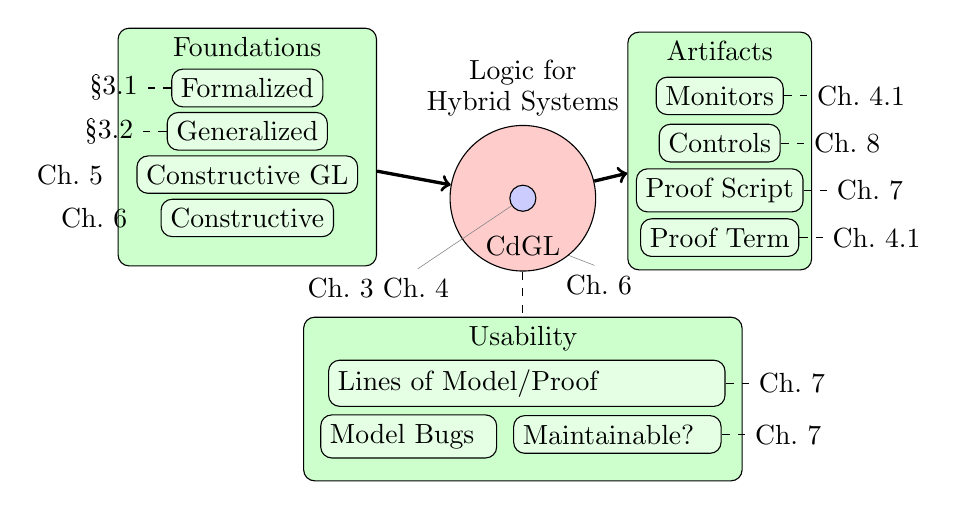
\begin{tikzpicture}[scale=0.5]
\draw (0,3.2)  node {Logic for};
\draw (0,2.4)  node {Hybrid Systems};
\draw (0,0)   node[circle]      (CdGLcirc) {\phantom{\hspace{1.1cm}}};
\draw (0,-1) node (cdgl) {\phantom{\CdGL}};
\node[coordinate,pin={[pin distance=0.55cm,text width=2cm]320:{Ch.\ 6}}] (cdgl-ref) at (cdgl) {};
\draw (0,0)   node[circle, fill=red!20,draw]      (CdGLcirc) {\phantom{\hspace{1.6cm}}};
\draw (0,-1.2) node (cdgl) {\CdGL};
\draw (0,0)   node[circle]  (dl)  {\phantom{\dL}};
\node[coordinate,pin={[pin distance=0.9cm,text width=3cm]265:{\ \ \ \ Ch.\ 3 Ch.\ 4}}] (dl-ref) at (dl) {};
\draw (dl) node[circle, fill=blue!20,draw]  {\dL};
\draw (-7, 1.3) node[rectangle,rounded corners,fill=green!20,draw,text depth=1in,text width=1.2in,text centered] (logic) {Foundations};
\draw (-7, 2.8) node[rectangle,rounded corners,fill=green!10,draw,thin,minimum height=0.3cm] (formalization) {\dL Formalized};
\draw (-7, 1.7) node[rectangle,rounded corners,fill=green!10,draw,thin,minimum height=0.3cm] (generalization) {\dL Generalized};
\draw (-7, 0.6) node[rectangle,rounded corners,fill=green!10,draw,thin,minimum height=0.3cm] (cgl) {Constructive \GL};
\draw (-7, -0.5) node[rectangle,rounded corners,fill=green!10,draw,thin,minimum height=0.3cm] (cdgl) {Constructive \dGL};
\draw node[left=0.3cm of formalization] (formal-ref) {\S3.1};
\draw node[left=0.3cm of generalization] (gen-ref) {\S3.2};
\draw node[left=0.3cm of cgl] (cgl-ref) {Ch.\ 5};
\draw node[left=0.3cm of cdgl] (cdgl-ref) {Ch.\ 6};
\draw[dashed] (formalization) -- (formal-ref);
\draw[dashed] (generalization) -- (gen-ref);
\draw (5, 1.2) node[rectangle,rounded corners,fill=green!20,draw,text depth=1in,text width=2.1cm,text centered] (engine) {Artifacts};
\draw (5, 2.6) node[rectangle,rounded corners,fill=green!10,draw,thin,minimum height=0.3cm] (monitors) {Monitors};
\draw (5, 1.4) node[rectangle,rounded corners,fill=green!10,draw,thin,minimum height=0.3cm] (controllers) {Controls};
\draw (5, 0.2) node[rectangle,rounded corners,fill=green!10,draw,thin,minimum height=0.3cm] (proofscript) {Proof Script};
\draw (5, -1) node[rectangle,rounded corners,fill=green!10,draw,thin,minimum height=0.3cm] (proofterm) {Proof Term};
\draw node[right=0.3cm of monitors] (monitor-ref) {Ch.\ 4.1};
\draw node[right=0.3cm of controllers] (controllers-ref) {Ch.\ 8};
\draw node[right=0.3cm of proofscript] (proofscript-ref) {Ch.\ 7};
\draw node[right=0.3cm of proofterm] (proofterm-ref) {Ch.\ 4.1};
\draw[dashed] (monitors) -- (monitor-ref);
\draw[dashed] (controllers) -- (controllers-ref);
\draw[dashed] (proofscript) -- (proofscript-ref);
\draw[dashed] (proofterm) -- (proofterm-ref);
\node[shape=coordinate] (use-anchor) at (0,-3){};
%\draw (1.45,-2) -- (0,-2.7);
\draw (0, -5.1) node[rectangle,rounded corners,fill=green!20,draw,text depth=1.6cm,text width=2.1in,text centered] (luser) {Usability};
%\draw (0, -3.1) node[rectangle,rounded corners,fill=green!10,draw,thin,minimum height=0.3cm] (monitors)    {Simplicity};
\draw (0.3, -4.7) node[rectangle,rounded corners,fill=green!10,draw,thin,minimum height=0.3cm] (monitors)    {Simplicity};
\draw (0.1, -4.7) node[rectangle,rounded corners,fill=green!10,draw,thin,minimum height=0.3cm,text width=4.8cm] (lop)    {Lines of Model/Proof};
%\draw (0, -4.15) node[rectangle,rounded corners,fill=green!10,draw,thin,minimum height=0.3in,text width=0.7in] (controllers) {Modeling Mistakes};
\draw (-2.9, -6.05) node[rectangle,rounded corners,fill=green!10,draw,thin,minimum height=0.3cm,text width=2cm] (modelmistake) {Model Bugs};
\draw (2.4, -6) node[rectangle,rounded corners,fill=green!10,draw,thin,minimum height=0.3cm,text width=2.4cm] (maintainable) {Maintainable?};
\draw node[right=0.3cm of maintainable] (maintain-ref) {Ch.\ 7};
\draw node[right=0.3cm of lop] (lop-ref) {Ch.\ 7};
\draw[->,very thick] (logic) -- (CdGLcirc);
\draw[->,very thick] (CdGLcirc) -- (engine);
\draw[dashed] (CdGLcirc) -- (luser);
\draw[dashed] (lop) -- (lop-ref);
\draw[dashed] (maintainable) -- (maintain-ref);
\end{tikzpicture}
\end{center}
%  \caption{Goals of the thesis}
%  \label{fig:goals-diagram}
%\end{figure}
\end{frame}
\section{Ongoing Work: \CdGL Logic}
% Say: CGL is already done, but for the sake of time we're presenting it together with CdGL
\begin{frame}[t]{Games Support Synthesis}
  \begin{tabular}{ccc}
    Modality                  & Curry-Howard & Synthesizes \\
    $\dbox{\alpha}{\phi}$     & Demon strategy for $\phi$ after $\alpha$ & Monitor \\
    $\ddiamond{\alpha}{\phi}$ & Angel strategy for $\phi$ after $\alpha$ & Control
  \end{tabular}\pause
  \begin{itemize}
  \item Games support monitor \emph{and} control synthesis from \emph{one} proof
  \item Curry Howard foundation promotes general-case, robust tools
  \item Game models are often simpler than systems
  \end{itemize}
\end{frame}

% Formula language, game language by Nim example, example properties
% Realizers, semantics
% quick 1-slide "proof terms exist"
% Soundness, prog+pres, implications for practice
% What's next: ODE's
\begin{frame}[t]{Nim Demonstrates Discrete Games}
  \begin{align*}
\turn &= \big\{\ptest{c>0};
                 \{\humod{c}{c-1} \cup \humod{c}{c-2} \cup \humod{c}{c-3}\};
                \ptest{c \geq 0}\big\};\\
\nim &=\Big\{\turn; \pdual{\turn}\Big\}\\
\textsf{Live} &\equiv c > 0 \limply \emod{c}{4} \neq 1 \limply \ddiamond{\prepeat{\nim}}{\bff}\\
\textsf{Safe} &\equiv c > 0 \limply \emod{c}{4} = 0 \limply \dbox{\drepeat{\nim}}{\,c = 0}
  \end{align*}
  \begin{itemize}
  \item $c \in \mathbb{N}$ counts remaining pebbles
  \end{itemize}
\end{frame}

\begin{frame}[t]{Realizers Capture Computation}
  \begin{align*}
\aa,\ab,\ac
&\bebecomes \rzBLam{\om}{f} \alternative \rzFOLam{x}{\tau}{\aa} \alternative \rzHOLam{x}{\phi}{\aa} \\
&\alternative  \rzNil \alternative \rzCons{\aa}{\ab}\alternative \rzApp{\aa}{v} \alternative \rzApp{\aa}{\ab} \alternative \rzApp{\aa}{\om} \alternative \rzFst{\aa} \alternative \rzSnd{\aa}
  \end{align*}
\begin{itemize}
  \item Semantics need to know: ``How does Angel make decisions?''
  \item Angel uses some base programming language $f$
  \item $\rzBLam{\om}{f}, \rzFOLam{x}{\tau}{\aa},$ and $\rzHOLam{x}{\phi}{\aa}$ take state $\om,$ base type $\tau,$ or proof parameters $\phi$, e.g., ``Demon told me how they proved $\phi$''
  \item Conjunctive proofs $\rzCons{\aa}{\ab},$ or nullary tuple $\rzNil$ when no choice needed
\end{itemize}
\end{frame}

\begin{frame}[t]{Formula Semantics}
\begin{itemize}
\item $\fintR{\phi}$ is the \emph{region} $X$ of strategy-state pairs $(\aa,\om)$ that realize $\phi$.
\item $\strategyforR[\alpha]{X}$ is the final region of game $\alpha$ starting from $X$ under Angel control
\item $\dstrategyforR[\alpha]{X}$ is the final region assuming \emph{Demon} control
\item Pseudo-state $\top$ indicates early success
\end{itemize}
\begin{align*}
(\rzNil,\om) \in  \fintR{f \geq g}                 &\text{ iff } \tint{f}{\om} \geq \tint{g}{\om}\\
(\aa,\om) \in  \fintR{\ddiamond{\alpha}{\phi}}       &\text{ iff } \strategyforR[\alpha]{\{(\aa,\om)\}} \subseteq (\fintR{\phi} \cup \{\stt\})\\
(\aa,\om) \in  \fintR{\dbox{\alpha}{\phi}}              &\text{ iff } \dstrategyforR[\alpha]{\{(\aa,\om)\}} \subseteq (\fintR{\phi} \cup \{\stt\})
\end{align*}
\end{frame}

\begin{frame}[t]{Angel Game Semantics}
\begin{align*}
\strategyforR[\ptest{\phi}]{X}            &= \{(\rzSnd{\aa},\om)~|~ (\aa,\om) \in X,~(\rzFst{\aa},\om) \in \fintR{\phi}\}\\
                                          &\cup \{\sff~|~(\aa,\om) \in X,~(\rzFst{\aa},\om) \notin \fintR{\phi}\}\\
\strategyforR[\humod{x}{f}]{X}  &= \{(\aa,\ssub{\om}{x}{\tint{f}{\om}})~|~(\aa,\om) \in X\}&&\text{}\\
\strategyforR[\prandom{x}]{X}          &= \{(\rzSnd{\aa},\ssub{\om}{x}{\rzFst{\aa}(\om)})~|~(\aa,\om) \in X\}&&\text{}\\
\strategyforR[\alpha;\beta]{X}           &= \strategyforR[\beta]{(\strategyforR[\alpha]{X})} &&\text{}\\
\strategyforR[\alpha\cup\beta]{X}      &= \strategyforR[\alpha]{\apL{X}} \cup \strategyforR[\beta]{\apR{X}}&&\text{}\\
\strategyforR[\prepeat{\alpha}]{X}     &= \bigcap\{\apL{Z}\subseteq \allRz \times \allstate~|~ X \cup (\strategyforR[\alpha]{\apR{Z}}) \subseteq Z\}
&&\\
\strategyforR[\pdual{\alpha}]{X}        &= (\dstrategyforR[\alpha]{X})&&\text{}
\end{align*}
\end{frame}

\begin{frame}[t]{Games Support Proof Terms}

\[M,N \bebecomes \edcase{A}{B}{C} \alternative \edinjL{A} \alternative \cdots \] % \ebcons{A}{B}
\pause
\cinferenceRule[dchoiceE|{$\langle\cup\rangle${E}}]{}
{
\linferenceRule[formula]
{\proves{\G}{A}{\ddiamond{\alpha\cup\beta}{\phi}}
        &\proves{\G,\pvl:\ddiamond{\alpha}{\phi}}{B}{\psi}
        &\proves{\G,\pvr:\ddiamond{\beta}{\phi}}{C}{\psi}}
{\proves{\G}{\edcase{A}{B}{C}}{\psi}}
}{}\\[0.1in]
\begin{calculuscollections}{\textwidth}
  \begin{calculus}
\cinferenceRule[dchoiceIL|{$\langle\cup\rangle${I1}}]{}
{\linferenceRule[formula]
  {\proves{\G}{M}{\ddiamond{\alpha}{\phi}}}
  {\proves{\G}{\edinjL{M}}{\ddiamond{\alpha\cup\beta}{\phi}}}
}{}
  \end{calculus}
  \begin{calculus}
\cinferenceRule[dchoiceIR|{$\langle\cup\rangle${I2}}]{}
{\linferenceRule[formula]
  {\proves{\G}{M}{\ddiamond{\beta}{\phi}}}
  {\proves{\G}{\edinjR{M}}{\ddiamond{\alpha\cup\beta}{\phi}}}
}{}
  \end{calculus}
\end{calculuscollections}\\[0.1in]
\pause
\begin{calculuscollections}{\textwidth}
  \begin{calculus}
\cinferenceRule[caseBetaL|{{case}$\beta$L}]{}{\edcase{\edinjL{A}}{B}{C} \stepsto \esub{B}{\ell}{A}}{}
\cinferenceRule[caseBetaR|{{case}$\beta$R}]{}{\edcase{\edinjR{A}}{B}{C} \stepsto \esub{C}{r}{A}}{}\pause
\cinferenceRule[caseS|caseS]{}{\linferenceRule[formula]
{\small{A \stepsto A'}}
{\small{\edcase{A}{B}{C} \stepsto \edcase{A'}{B}{C}}}}{}
  \end{calculus}
\end{calculuscollections}
\end{frame}

\begin{frame}[t]{Sound as a Logic}
\begin{lemma}[Renaming]
  If $\proves{\G}{M}{\phi}$ then $\proves{\esub{\G}{x}{y}}{\esub{M}{x}{y}}{\esub{\phi}{x}{y}}$.
\end{lemma}
\begin{lemma}[Context substitution]
  If $\proves{\G,x:\psi}{M}{\phi}$ and $\proves{\G}{N}{\psi}$ then $\proves{\G}{\esub{M}{x}{N}}{\phi}$.
\end{lemma}
\begin{lemma}[Variable substitution]
  If $\proves{\G}{M}{\phi}$ and $\esub{\phi}{x}{\theta}$ is admissible then $\proves{\esub{\G}{x}{\theta}}{\esub{M}{x}{\theta}}{\esub{\phi}{x}{\theta}}$.
\end{lemma}
\begin{theorem}[Soundness of Proof Calculus]
  If $\proves{\cdot}{M}{\phi}$ then $\phi$ is realizability-valid.
\end{theorem}
\end{frame}

\begin{frame}[t]{Sound as a Type System}
\begin{lemma}[Progress]
If $\proves{\Gamma}{M}{\phi},$ then either $M$ is normal or $M \stepsto N$ for some $N$.
\end{lemma}
\begin{lemma}[Preservation]
If $\proves{\Gamma}{M}{\phi}$ and $M \stepsto^* N,$ then $\proves{\Gamma}{N}{\phi}$
\end{lemma}
\begin{lemma}[Existence Property]
If $\proves{\Gamma}{M}{(\lexists{x:\tau}{\phi})}$ then there exists a term $f$ and realizer $\ab$ such that for all $(\aa,\om) \in \cintR{\G},$
we have $(\rzApp{\ab}{\aa},\ssub{\om}{x}{f(\om)}) \in \fintR{\phi}$.
\label{lem:term-ep}
\end{lemma}
\begin{lemma}[Disjunction Property]
When $\proves{\Gamma}{M}{\phi \lor \psi}$ there exists realizer $\ab$ and computable $f,$ s.t.\ for every $\om$ and $\aa$ such that $(\aa,\omega) \in \cintR{\G}$, either $f(\omega)=0$ and $(\rzFst{\ab},\omega) \in \fintR{\phi}{}$, else $f(\omega)=1$ and $(\rzSnd{\ab},\omega) \in \fintR{\psi}$.
\end{lemma}
%\begin{lemma}[Active Strategy Property]
%If $\proves{\Gamma}{M}{\ddiamond{\alpha}{\phi}},$ then there exists a realizer $\ab$ such that for all $\om$ and realizers $\aa$ such that $(\aa,\om) \in \cintR{\G},$
%then $\strategyforR[\alpha]{\{(\rzApp{\ab}{\aa},\om)\}} \subseteq \fintR{\phi} \cup \{\stt\}$.
%\end{lemma}
\end{frame}

\begin{frame}[t]{Proposed Work: ODE's}
Picard iteration and Euler integration yield computational interpretations of ODE's.
\begin{itemize}
  \item Application: Euler proofs of $\ddiamond{\pevolve{\D{x}=\theta}}{P}$ support synthesis of Model-Predictive Control
  \item Conjecture: Box rules $\dbox{\pevolve{\D{x}=\theta}}{P}$ ``just work''
  \item Challenge: Which proofs lead to ``good'' monitors, controllers?
     e.g., equalities $\theta = \eta$ are easy to prove, hard to monitor.
  \item Related Work: Verified integration~\cite{DBLP:conf/itp/ImmlerT16}
\end{itemize}
\end{frame}

\begin{frame}[t]{Proposed Work: Connections}
How do games connect with systems, and thus with VeriPhy?\\
\begin{itemize}
\item Extend differential refinement logic \dRL to games
\item Make folk theorem rigorous: ``Games $\equiv$ Systems $\mod$ Strategies"
\end{itemize}
\pause
How do constructive and classical games relate?
\begin{itemize}
\item G\"{o}del-Gentzen translation and embedding classical proofs ``as a modality''
\item Conjecture: Classical games are ``bigger'' (higher closure ordinal) than constructive games
\item Expand study of classical vs.\ constructive arithmetic
\end{itemize}
\end{frame}

\section{Proposed Work: Kaisar Language}

\begin{frame}[t]{Kaisar Combines Perspectives on Proofs}
  \begin{tabular}{lll}
    \ah{1}{\engineer}                         & \ah{2}{\logician}                      & \ah{3}{\logicuser}\\
    \acl{1}{\say{Can it synthesize?}} & \acl{2}{\say{What \emph{is} a program proof?}} & \acl{3}{\say{Does it scale?}}
  \end{tabular}
\end{frame}

%TODO: Give actual examples and motivations for nominals
\begin{frame}[t,fragile]{Programs First, Proofs Second}
\logician[0.5in]
\begin{minipage}{2in}
\begin{verbatim}
     (x:=1 {show (x > 0) using x by auto})
U   (x:= 2 {show (x > 0) using x by auto})
\end{verbatim}
\end{minipage}
\begin{minipage}{2in}
\begin{verbatim}
(x:=1 U  x:=2)
{show (x > 0) using x by auto}
\end{verbatim}
\end{minipage}

\begin{verbatim}
x:=2;
{x:=x+1}*\@{show gr1:"x>1" using x by auto}
{show "x>0" using gr1 by auto}
\end{verbatim}

\end{frame}

%TODO: More Logic-User slides?
\begin{frame}[t]{Evaluation}
\logicuser[0.5in] 
Best-effort usability eval.\ for lightweight design guidance
\begin{itemize}
\item Maintenance: How do proofs change when programs change?
\item Concision: How do ports of old proofs compare to originals?
\item Proof Patterns: Identify common idioms. Are they easy to express?
\end{itemize}
\end{frame}

%TODO: Change example to support the idioms
\begin{frame}[t]{Logic-User is Hopeful}
  \begin{itemize}
  \item Nominals support ``predictive proof'' idiom
  \item Lexical scope taken for granted in programs
  \item Nominals underly abstractions which support maintenance
  \item Deduplication is essential for concision
  \end{itemize}
\end{frame}

%TODO: Read up on bifurcations
\begin{frame}[t]{Theory Supports Design Goals}
\logician[0.5in]
How much do proofs change when programs change?
\begin{itemize}
\item Intimately related to proof modularity
\item Identify an interface $D(\beta)$ of facts about subprogram $\beta$ of theorem $C(\beta)$
\item A modular proof $F$ uniformly proves $D(\gamma) \limply C(\phi)$ for \emph{all} $\gamma$
\item Smaller $D$ means more modular
\item Compare: ``Adaptation completeness'' in Vienna Development Method
\end{itemize}
\end{frame}

\begin{frame}[t]{Predicate Transformers Meet Hybrid Logic}
\logician[0.5in]
How do we check proofs?
How do we trust proofs?

Compute strongest postcondition $\spost{S}{\G}$ of proof $S$ from initial context $\G$.
\begin{align*}
\spost{\{\sshow{x}{\phi}{U}\}}{\G}             &= \phi                                        &&\text{if U proves }\phi\\
\spost{\{\shave{x}{\phi}{U}{S}\}}{\G}          &= \spost{S}{(\G,x:\phi)}                      &&\text{if U proves }\phi\\
\spost{\alpha;\beta}{\G}                       &= \spost{\beta}{(\G_\alpha,\spost{\alpha}{\G})} &&\\
\spost{\alpha\cup\beta}{\G}                    &= \spost{\alpha}{\G} \vee \spost{\beta}{\G}   &&\\
\spost{?(x:\phi)}{\G} &= \phi &&\\
\spost{\humod{x}{\theta}}{\G} &=(x=\theta) &&\\
  \spost{(\alpha)^*@\{B\}}{\G} &= \spost{\{B\}}{G} &&\text{if }\spost{\alpha}{{\G_\alpha}_{\{B\}}}=\spost{\{B\}}{\G}\\
\spost{L{:}\ \alpha}{\G} &= \spost{\alpha}{(\G,L)}
\end{align*}
\textbf{Soundness:} If $S$ is a proof, then $\G \vdash \spost{S}{\G}$ is valid.
\end{frame}

\begin{frame}[t]{Kaisar as a Playground}
Proof technology has evolved over time.
Let's answer:
  \begin{tabular}{lll}
    \ah{1}{\engineer}                         & \ah{2}{\logician}                      & \ah{3}{\logicuser}\\
    \acl{1}{\say{How does proof format affect tooling?}} 
& \acl{2}{\say{What are the core features?}}
& \acl{3}{\say{How do features impact real proofs?}}
  \end{tabular}
\end{frame}

\section{Proposed Work: Controller Synthesis}

\begin{frame}[t]{Exploit Proof Content}
\end{frame}

\begin{frame}[t]{Architecture}
\end{frame}

\begin{frame}[t]{Arithmetic}
\end{frame}

\begin{frame}[t]{Code Generation}
\end{frame}

\begin{frame}[t]{}
\end{frame}

\section{Conclusion}
\begin{frame}[t]{}
  
\end{frame}

\appendix
\section<presentation>*{\appendixname}
\subsection<presentation>*{For Further Reading}

\begin{frame}[t, allowframebreaks]
\frametitle{References}
\bibliographystyle{amsalpha}
\bibliography{proposal,platzer,verified-pipeline,hilbert-epsilons,ground-robotics,verified-dL,constructive-games,kaisar}
\end{frame}

\end{document}